\documentclass{report}
\usepackage{graphicx}
\usepackage{hyperref}
\usepackage{float}

\begin{document}
	
	% --- Cover Page ---
	\begin{titlepage}
		\centering
		
\includegraphics[width=4cm]{icon_ku.png}\par\vspace{2cm}
		{\Huge \bfseries Accommodation Services: Occurrence Booking System\par}
		\vspace{1cm}
		{\Large User \& Administrator Manual\par}
		\vfill
		Prepared by IT Department\par
		\today
	\end{titlepage}
	
	% --- Table of Contents ---
	\tableofcontents
	\newpage
	

	\chapter{Login Page}
	
	When you visit the system at \url{https://aobs.ku.ac.ke/}, you are directed to the login page.
	
	\begin{figure}[h!]
		\centering
		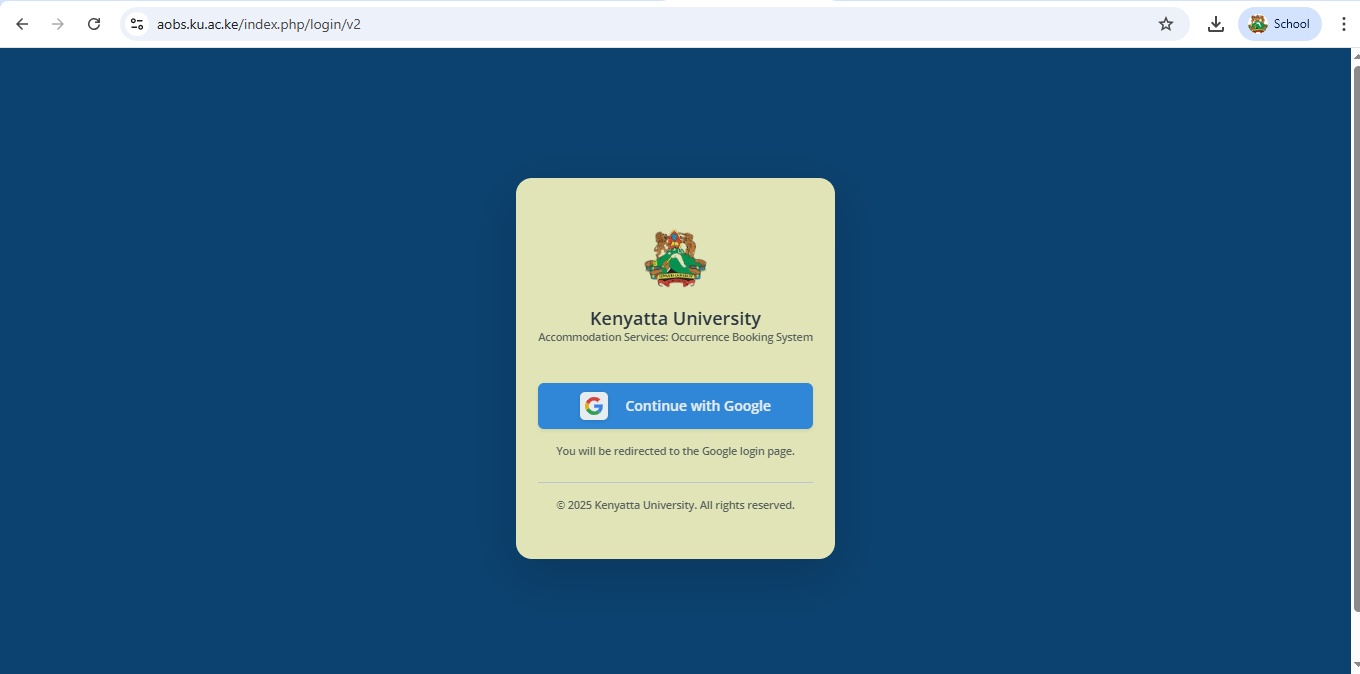
\includegraphics[width=0.7\textwidth]{screenshots/login.png} % <-- replace with your screenshot filename
		\caption{System Login Page (Google Sign-In Only)}
		\label{fig:login}
	\end{figure}
	
	\section*{Description}
	The system uses \textbf{Google Authentication} for login.  
	\begin{itemize}
		\item Users must click the \textbf{Login with Google} button.  
		\item The system will redirect them to their Google account for authentication.  
		\item After successful verification, users are redirected to the \textbf{Dashboard}.  
	\end{itemize}
	
	\section*{Roles}
	\begin{itemize}
		\item \textbf{Administrators} log in via their institutional Google accounts.  
		\item \textbf{Staff/Users} log in with their institutional Google accounts.  
	\end{itemize}
	
	\section*{Security Features}
	\begin{itemize}
		\item Password management is handled by \textbf{Google} (the system does not store user passwords).  
		\item Only authorized Google accounts are allowed access.  
		\item Failed or unauthorized attempts are logged for auditing.  
	\end{itemize}
	
	
	\chapter{System Navigation}
	
	After logging in successfully, users are directed to their respective \textbf{Dashboard}.  
	From the dashboard, all system features are accessed using the left-side \textbf{Navigation Menu}.  
	
	\section*{Navigation for Users with access to entire system}
	Administrators, Coordinators, Zonal Officers, Directors, Managers, and all other users except Hostel Attendants and Housekeepers will see the following menu items:
	
	\begin{itemize}
		\item \textbf{Dashboard} -- Overview of system activity.  
		\item \textbf{User} -- Manage system users.  
		\item \textbf{Occurrence} -- Record and review occurrences.  
		\item \textbf{Zones} -- Manage geographical zones.  
		\item \textbf{Hostels} -- Manage hostel details.  
		\item \textbf{Reports} -- Access different report types:  
		\begin{itemize}
			\item All Reports  
			\item Add Report  
			\item Zonal Reports  
			\item Administrator/Coordinator Reports  
		\end{itemize}
		\item \textbf{Student Statistics} -- View student-related statistics.  
		\item \textbf{Escalation Matrix} -- Manage escalation contacts and workflow.  
		\item \textbf{Escalations} -- Track escalated cases.  
		\item \textbf{Handover/Takeover} -- Manage shift changes.  
	\end{itemize}
	
	\begin{figure}[h!]
		\centering
		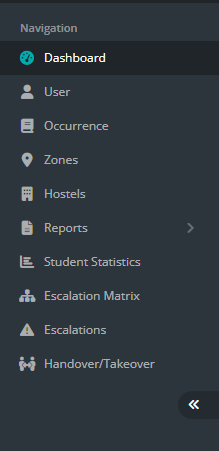
\includegraphics[width=0.25\textwidth]{screenshots/navigation_admin.png} % <-- your screenshot here
		\caption{Navigation Menu for Administrators and General Users}
		\label{fig:nav-admin}
	\end{figure}
	
	\section*{Navigation for Hostel Attendants and Housekeepers}
	Attendants and Housekeepers have a simplified menu with only the relevant features:
	
	\begin{itemize}
		\item \textbf{Dashboard} -- Personalized dashboard.  
		\item \textbf{Occurrence} -- Record daily occurrences.  
		\item \textbf{Student Statistics} -- View student-related statistics.  
		\item \textbf{Handover/Takeover} -- Manage daily shift transitions.  
	\end{itemize}
	
	
	
	\section*{How to Use the Navigation Menu}
	\begin{enumerate}
		\item Move your cursor to the left sidebar.  
		\item Click a menu item to open the corresponding page.  
		\item Sub-menus (e.g., Reports) expand when clicked.  
		\item Use the back button or dashboard link to return to the main page.  
	\end{enumerate}
	
	
	
	\chapter{User Management}
	
	The User module allows authorized staff to view, create, update, and manage system users.  
	Only Administrators, Coordinators, Managers, and Directors have permission to access this module.  
	
	\section*{User List}
	When you click on the \textbf{User} menu item, the system shows a list of all registered users.  
	The table contains the following columns:  
	\begin{itemize}
		\item \textbf{\#} – Serial number.  
		\item \textbf{Name} – Full name of the user.  
		\item \textbf{Email} – Email address used for Google login.  
		\item \textbf{Phone} – Contact phone number (if provided).  
		\item \textbf{Role} – User role, displayed as a colored badge (e.g., Administrator, Manager, Director).  
		\item \textbf{Created At} – Date and time when the account was created.  
		\item \textbf{Actions} – Buttons to \textbf{Edit} or \textbf{Delete} the user.  
	\end{itemize}
	
	\begin{figure}[h!]
		\centering
		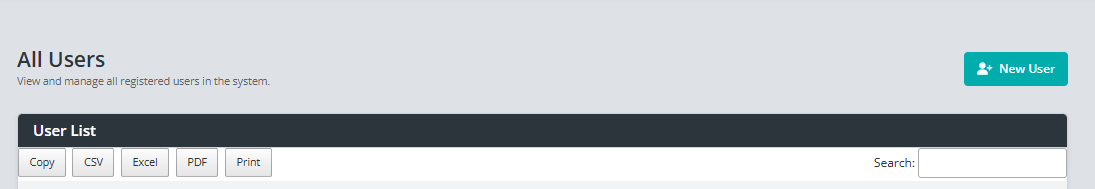
\includegraphics[width=1.2\textwidth]{screenshots/user_list.png}
		\caption{User List with Actions}
		\label{fig:user-list}
	\end{figure}
	
	\section*{Creating a New User}
	Click the \textbf{New User} button above the user table to open the user creation form.  
	
	The form contains the following fields:  
	\begin{itemize}
		\item \textbf{Name} – Full name of the new user.  
		\item \textbf{Email} – Institutional Google email address.  
		\item \textbf{Phone} – Contact number (optional).  
		\item \textbf{Role} – Role of the user (Administrator, Coordinator, Zonal Officer, Director, Manager, House Keeper, Hostel Attendant, or Other).  
		\item \textbf{Other Role} – If “Other” is selected, specify the role manually.  
	\end{itemize}
	
	Once all details are filled, click \textbf{Create User} to register the account.  
	Success or error messages are displayed at the top of the form.  
	
	\begin{figure}[h!]
		\centering
		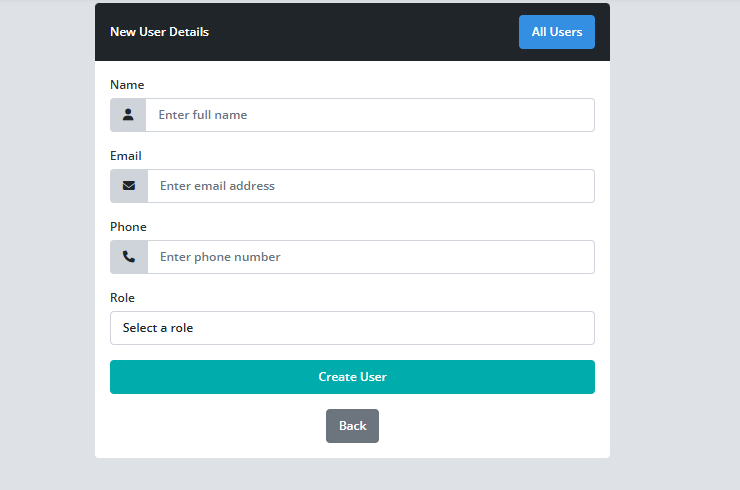
\includegraphics[width=0.8\textwidth]{screenshots/user_new.png}
		\caption{New User Creation Form}
		\label{fig:user-new}
	\end{figure}
	
	\section*{Editing a User}
	To update a user, click the \textbf{Edit} button in the User List.  
	This opens the Edit User form, where you can:  
	\begin{itemize}
		\item Modify \textbf{Name}, \textbf{Email}, or \textbf{Phone}.  
		\item Change the \textbf{Role} (only visible for Managers or Directors).  
		\item Save changes by clicking the \textbf{Update User} button.  
	\end{itemize}
	
	\begin{figure}[h!]
		\centering
		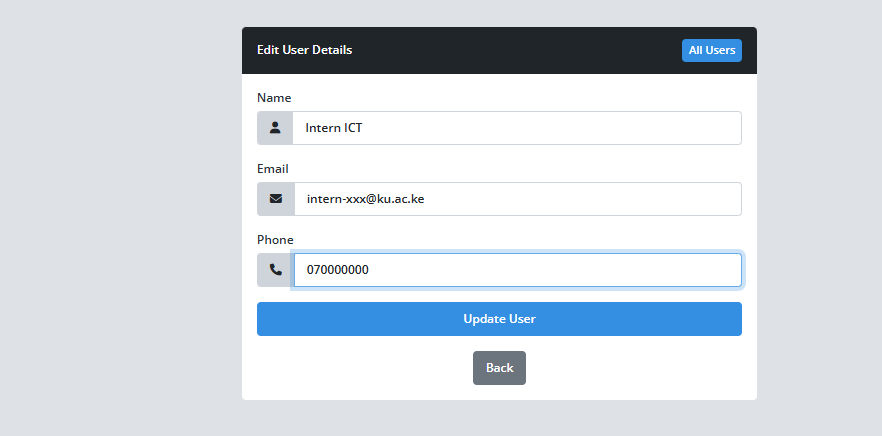
\includegraphics[width=0.8\textwidth]{screenshots/user_edit.png}
		\caption{Editing User Details}
		\label{fig:user-edit}
	\end{figure}
	
	\section*{Deleting a User}
	The \textbf{Delete} button in the Actions column allows removal of a user.  
	\begin{itemize}
		\item A confirmation prompt appears before deletion.  
		\item Once deleted, the user account cannot log in again.  
		\item However, their past records remain in reports for accountability.  
	\end{itemize}
	
	\section*{Notes}
	\begin{itemize}
		\item User accounts must have a valid institutional Google email.  
		\item Roles determine the system features available to each user.  
		\item Administrators are responsible for maintaining correct user roles.  
	\end{itemize}
	
	
	\chapter{Zone Management}
	
	
	This module allows authorized users to create, view, and manage zones.  
	
	
	\section*{Zones List}
	Click the \textbf{Zones} menu item to open the list of registered zones.  
	The table includes the following columns:
	\begin{itemize}
		\item \textbf{\#} – Serial number.
		\item \textbf{Zone Name} – The name of the zone.
		\item \textbf{Actions} – Buttons to edit (and optionally delete) the zone.
	\end{itemize}
	
	If no zones exist, the system displays a “No zones found” message.
	
	\begin{figure}[h!]
		\centering
		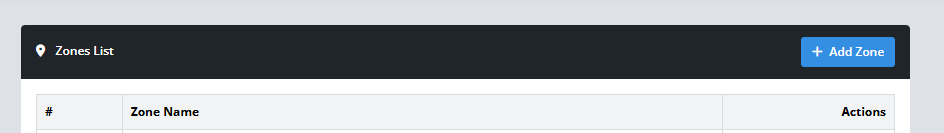
\includegraphics[width=\textwidth]{screenshots/zones_list.png}
		\caption{Zones List with Actions}
		\label{fig:zones-list}
	\end{figure}
	
	\section*{Adding a New Zone}
	Click the \textbf{Add Zone} button to create a new zone.  
	This opens a form requiring the following field:
	\begin{itemize}
		\item \textbf{Zone Name} – The name of the new zone (required).
	\end{itemize}
	
	At the bottom of the form:
	\begin{itemize}
		\item Click \textbf{Save Zone} to create the record.
		\item Click \textbf{Cancel} to return to the list without saving.
	\end{itemize}
	
	Validation ensures that the name field is not left blank.  
	If successful, a success message is displayed.
	
	\begin{figure}[h!]
		\centering
		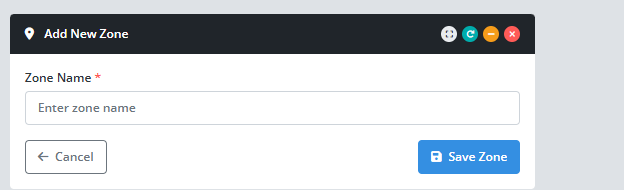
\includegraphics[width=0.9\textwidth]{screenshots/zones_add.png}
		\caption{Add New Zone Form}
		\label{fig:zones-add}
	\end{figure}
	
	\section*{Editing a Zone}
	To update an existing zone:
	\begin{enumerate}
		\item From the Zones List, click the \textbf{Edit} button in the Actions column.
		\item The Edit Zone form appears with the current name pre-filled.
		\item Modify the \textbf{Zone Name} as required.
		\item Click \textbf{Update Zone} to save changes or \textbf{Cancel} to discard.
	\end{enumerate}
	
	If validation fails, error messages appear above the form.
	
	\begin{figure}[h!]
		\centering
		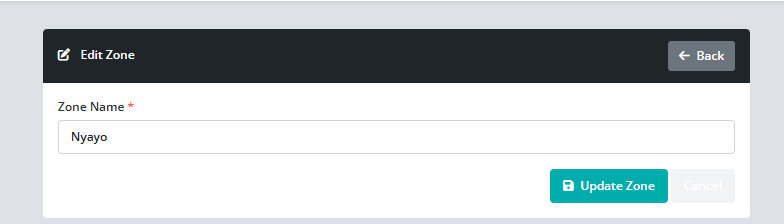
\includegraphics[width=0.9\textwidth]{screenshots/zones_edit.png}
		\caption{Edit Zone Form}
		\label{fig:zones-edit}
	\end{figure}
	
	\section*{Notes}
	\begin{itemize}
		\item Zones are important for grouping hostels and assigning responsibilities to zonal officers.
		\item Deletion of zones may be disabled to protect historical records.
	\end{itemize}
	
	\chapter{Hostel Management}
	
	The Hostel module allows Administrators and Coordinators to create, edit, and manage hostels within different zones.  
	Each hostel is associated with a zone and has a defined student capacity.
	
	\section*{Hostels List}
	Click the \textbf{Hostels} menu item to view all registered hostels.  
	The table shows:
	\begin{itemize}
		\item \textbf{\#} – Serial number.
		\item \textbf{Hostel Name} – The name of the hostel.
		\item \textbf{Zone} – The zone to which the hostel belongs.
		\item \textbf{No. of Students} – The total capacity (or current number of students).
		\item \textbf{Actions} – Edit (and optionally delete) buttons.
	\end{itemize}
	
	If no hostels are available, the system displays a message: “No hostels found.”
	
	\begin{figure}[h!]
		\centering
		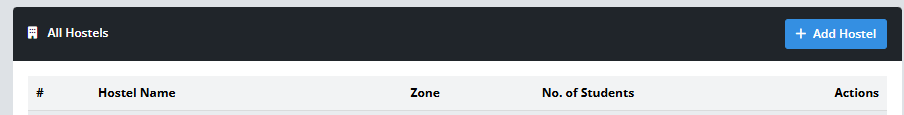
\includegraphics[width=\textwidth]{screenshots/hostels_list.png}
		\caption{Hostels List with Actions}
		\label{fig:hostels-list}
	\end{figure}
	
	\section*{Adding a New Hostel}
	Click the \textbf{Add Hostel} button to open the form. The following fields are required:
	\begin{itemize}
		\item \textbf{Hostel Name} – Enter the hostel’s name.
		\item \textbf{Zone} – Select the zone to which the hostel belongs.
		\item \textbf{Number of Students (Capacity)} – Define the hostel’s capacity.
	\end{itemize}
	
	At the bottom:
	\begin{itemize}
		\item Click \textbf{Save Hostel} to create the hostel.
		\item Click \textbf{Cancel} to return to the hostels list without saving.
	\end{itemize}
	
	\begin{figure}[h!]
		\centering
		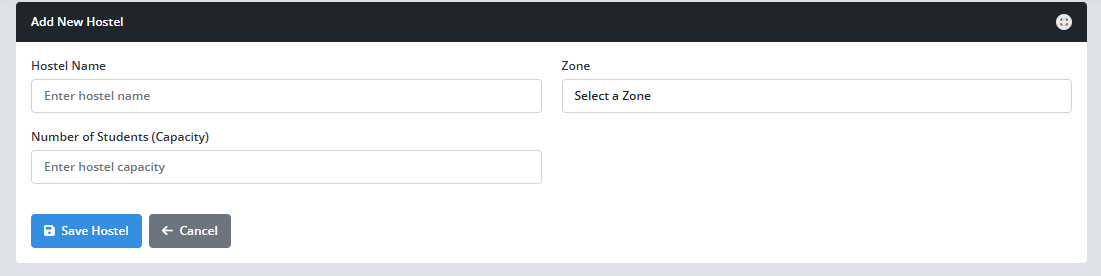
\includegraphics[width=0.9\textwidth]{screenshots/hostels_add.png}
		\caption{Add New Hostel Form}
		\label{fig:hostels-add}
	\end{figure}
	
	\section*{Editing a Hostel}
	To update a hostel:
	\begin{enumerate}
		\item In the Hostels List, click the \textbf{Edit} button from the Actions column.
		\item The Edit Hostel form opens with the details pre-filled.
		\item Update the fields (Zone, Hostel Name, Capacity).
		\item Click \textbf{Update Hostel} to save changes, or \textbf{Back} / \textbf{Cancel} to exit without saving.
	\end{enumerate}
	
	Validation messages are displayed if required fields are left empty.
	
	\begin{figure}[h!]
		\centering
		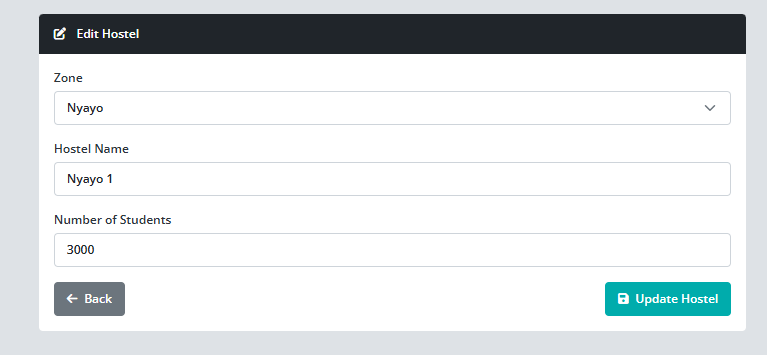
\includegraphics[width=0.9\textwidth]{screenshots/hostels_edit.png}
		\caption{Edit Hostel Form}
		\label{fig:hostels-edit}
	\end{figure}
	
	\section*{Notes}
	\begin{itemize}
		\item Every hostel must belong to a zone.
		\item Capacity is a mandatory field to ensure proper allocation of students.
		\item Deletion of hostels may be restricted to protect historical allocation data.
	\end{itemize}
	
	
	
	
	\chapter{Occurrence Management}
	
	The Occurrence module is used to report, track, escalate, and resolve incidents happening in hostels.  
	Occurrences go through multiple steps: reporting, action, escalation, and resolution.
	
	\section*{All Occurrences}
	Click \textbf{Occurrences} on the navigation menu to see a full list of all reported occurrences.  
	The table displays:
	\begin{itemize}
		\item \textbf{Tracking Number} – A unique reference for the occurrence.
		\item \textbf{User} – The staff member who reported.
		\item \textbf{Shift} – Day or Night.
		\item \textbf{Hostel} – The hostel where the incident occurred.
		\item \textbf{Date, Time of Reporting, Time of Occurrence}.
		\item \textbf{Occurrence Type, Nature, Action Taken, Resolution, Resolved}.
		\item \textbf{Files} – Any supporting attachments.
		\item \textbf{Stakeholder Inputs} – Comments/inputs from hostel attendants, zonal officers, administrators, managers, and directors.
	\end{itemize}
	
	From this page, users can:
	\begin{itemize}
		\item \textbf{Add a new occurrence}.
		\item \textbf{Escalate an occurrence}.
		\item (Higher roles) \textbf{Edit or delete an occurrence}.
		\item Add \textbf{inputs/comments}.
	\end{itemize}
	
	\begin{figure}[h!]
		\centering
		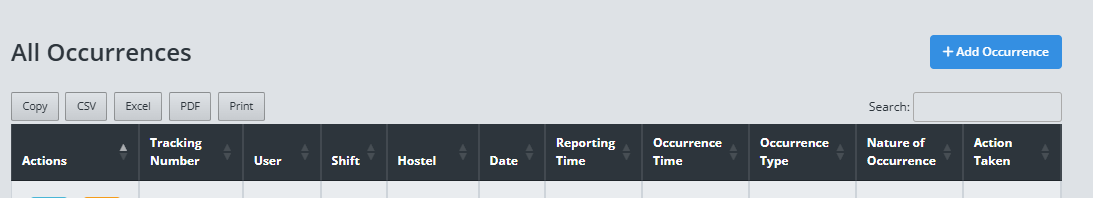
\includegraphics[width=\textwidth]{screenshots/occurrences_list.png}
		\caption{Occurrences List with Actions}
		\label{fig:occurrences-list}
	\end{figure}
	
	\section*{Reporting a New Occurrence}
	Click \textbf{Add Occurrence} to launch a multi-step wizard:
	\begin{enumerate}
		\item \textbf{Step 1 – Reporter Details:} The system auto-fills your name and role. Select shift and hostel.
		\item \textbf{Step 2 – Occurrence Details:} Fill date, time of reporting, occurrence time, type of occurrence (choose from list or specify "Other"), and describe the nature of the incident.
		\item \textbf{Step 3 – Actions:} Record the action taken, mark whether resolved, provide resolution details, and upload supporting files.
	\end{enumerate}
	
	Navigation buttons (\textbf{Previous}, \textbf{Next}, \textbf{Submit}) guide you through the process.
	
	\begin{figure}[h!]
		\centering
		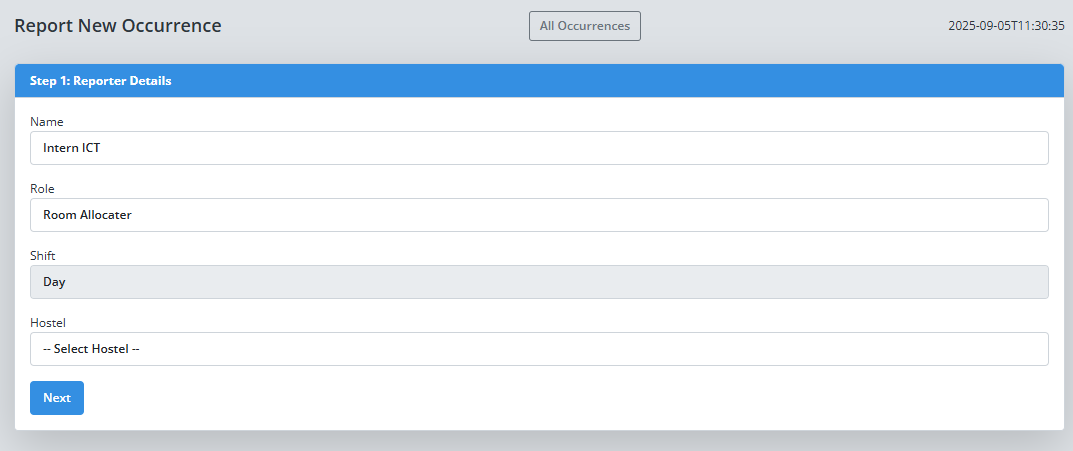
\includegraphics[width=\textwidth]{screenshots/occurrence_create.png}
		\caption{Report New Occurrence Form}
		\label{fig:occurrence-create}
	\end{figure}
	
	
	
	\section*{Occurrence Details View}
	Click a tracking number to view the full occurrence details.  
	This page is organized into tabs:
	\begin{itemize}
		\item \textbf{Occurrence Details} – Reporter, shift, hostel, date/time, type, resolution status.
		\item \textbf{Escalations} – Escalation history.
		\item \textbf{Resolution} – Resolution records.
		\item \textbf{Stakeholder Inputs} – Comments from staff across different roles.
		\item \textbf{Files} – Uploaded supporting files.
	\end{itemize}
	
	\begin{figure}[h!]
		\centering
		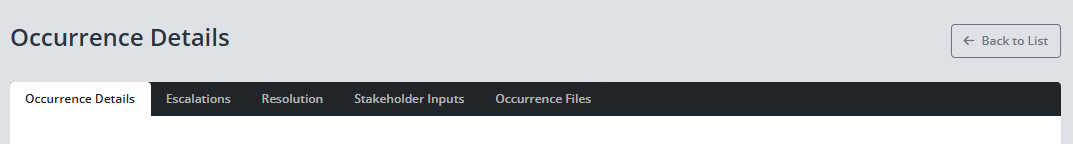
\includegraphics[width=\textwidth]{screenshots/occurrence_details.png}
		\caption{Occurrence Details Tabs}
		\label{fig:occurrence-details}
	\end{figure}
	
	\section*{Escalations and Inputs}
	Every occurrence can be escalated to higher roles for further action.  
	Users can also add inputs (comments or observations). Inputs are tagged with the user’s role and name.  
	
	\section*{Notes}
	\begin{itemize}
		\item Only authenticated users can report occurrences.
		\item Role determines access: attendants and housekeepers mainly report, while zonal officers, administrators, managers, and directors escalate, update, or close reports.
		\item Attachments can include documents, images, or PDFs.
	\end{itemize}
	
	
	
	\chapter{Daily Reports}
	
	The Daily Reports module allows hostel staff and zonal officers to submit and review daily activity reports.  
	Managers and Directors can also add their inputs to each report.
	
	\section*{All Reports}
	Click \textbf{Reports} on the navigation menu to see all submitted reports.  
	The reports table shows the following information:
	\begin{itemize}
		\item \textbf{Date \& Time} – When the report was submitted.
		\item \textbf{Report} – The detailed text entered by the user.
		\item \textbf{Shift} – Day or Night.
		\item \textbf{Zone} – The zone associated with the report (for zonal officers).
		\item \textbf{System User} – The staff member who submitted the report.
		\item \textbf{Manager Input} – Notes or comments from the Manager (if any).
		\item \textbf{Director Input} – Notes or comments from the Director (if any).
	\end{itemize}
	
	If you are a \textbf{Manager} or \textbf{Director}, you will see action buttons next to each report, allowing you to:
	\begin{itemize}
		\item Add your input (via the comment icon).
		\item (Optional) Edit or delete a report (if permissions allow).
	\end{itemize}
	
	\begin{figure}[h!]
		\centering
		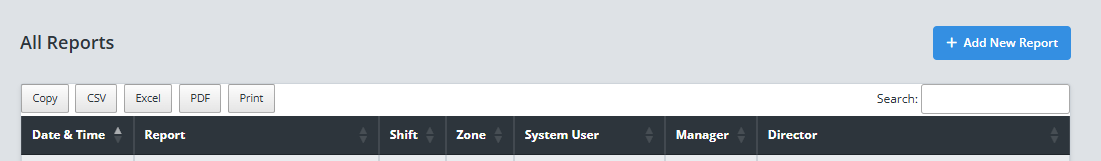
\includegraphics[width=\textwidth]{screenshots/reports_list.png}
		\caption{All Daily Reports List}
		\label{fig:reports-list}
	\end{figure}
	
	\section*{Adding a New Report}
	To submit a report, click the \textbf{Add New Report} button at the top-right of the Reports page.  
	This opens the Daily Report Form.
	
	\begin{enumerate}
		\item \textbf{Zone} – Required for Zonal Officers. Select from the dropdown list.
		\item \textbf{Date \& Time} – Specify when the report was made.
		\item \textbf{Shift} – Day or Night (auto-selected by the system).
		\item \textbf{Report} – Enter the full details of the daily report in the textarea provided.
	\end{enumerate}
	
	After completing the form, click \textbf{Submit Report}.  
	The system will save your entry and display it in the reports list.
	
	\begin{figure}[h!]
		\centering
		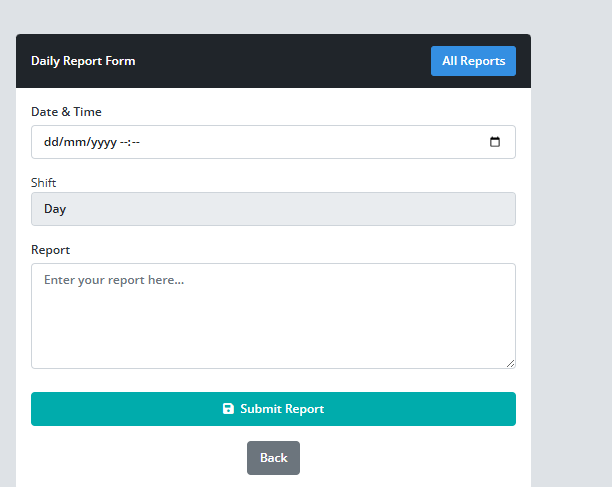
\includegraphics[width=0.95\textwidth]{screenshots/report_create.png}
		\caption{Daily Report Submission Form}
		\label{fig:report-create}
	\end{figure}
	
	\section*{Adding Inputs (Manager \& Director)}
	Managers and Directors can add comments or approvals to submitted reports.  
	Click the \textbf{Add Input} button (speech bubble icon) next to the relevant report.  
	A modal will appear where you can type and save your input.
	
	\begin{figure}[h!]
		\centering
		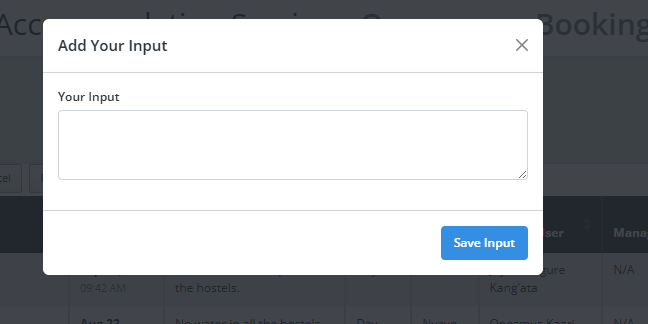
\includegraphics[width=0.8\textwidth]{screenshots/report_input_modal.png}
		\caption{Add Manager/Director Input to a Report}
		\label{fig:report-input}
	\end{figure}
	
	\section*{Notes}
	\begin{itemize}
		\item Only authorized users can submit daily reports.
		\item Managers and Directors have additional privileges to comment on reports.
		\item Reports are permanently stored and can be used for accountability and auditing.
	\end{itemize}
	
	
	
	\chapter{Student Attendance Statistics}
	
	This module is used to record and monitor student attendance in each hostel.  
	It helps administrators, zonal officers, and other staff members keep accurate statistics of students present during different shifts.
	
	\section*{Viewing Attendance Records}
	Click \textbf{Student Attendance Statistics} from the navigation menu to view all submitted records.  
	The table displays the following information:
	\begin{itemize}
		\item \textbf{Reported By} – The staff member who recorded the statistics.
		\item \textbf{Hostel} – The hostel where attendance was taken.
		\item \textbf{Zone} – The zone of the hostel.
		\item \textbf{Date} – Date of the record.
		\item \textbf{Shift} – Day or Night.
		\item \textbf{Students Present} – The total number of students present.
		\item \textbf{Comments} – Any remarks or additional notes.
	\end{itemize}
	
	\begin{figure}[h!]
		\centering
		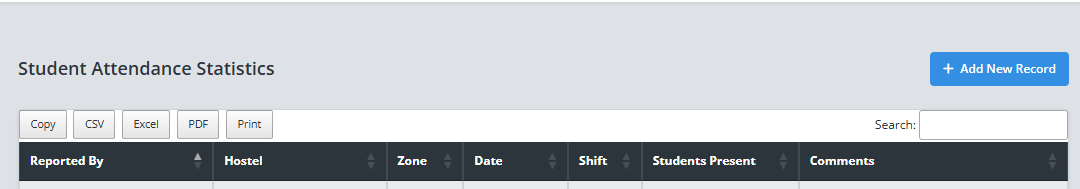
\includegraphics[width=\textwidth]{screenshots/student_statistics_list.png}
		\caption{Student Attendance Statistics List}
		\label{fig:student-statistics-list}
	\end{figure}
	
	\section*{Adding a New Record}
	To add a new attendance record, click the \textbf{Add New Record} button at the top-right of the Student Attendance Statistics page.  
	This will open the Student Statistics Form.
	
	The form contains the following fields:
	\begin{enumerate}
		\item \textbf{Hostel} – Select the hostel from the dropdown list.
		\item \textbf{Date of Record} – The date when attendance is recorded.
		\item \textbf{Shift} – Select Day or Night.
		\item \textbf{Students Present} – Enter the total number of students present.
		\item \textbf{Comments} – (Optional) Add any notes or observations.
	\end{enumerate}
	
	After filling in the details, click \textbf{Save Record} to submit.  
	The system validates the data before saving and will display any error messages if required fields are missing.
	
	\begin{figure}[h!]
		\centering
		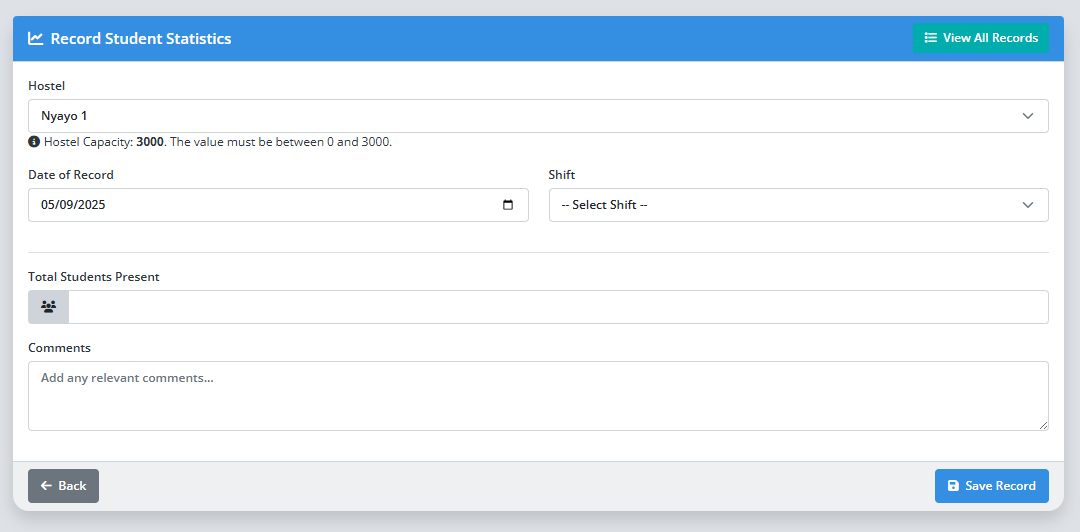
\includegraphics[width=0.95\textwidth]{screenshots/student_statistics_form.png}
		\caption{Student Attendance Statistics Form}
		\label{fig:student-statistics-form}
	\end{figure}
	
	\section*{Permissions}
	\begin{itemize}
		\item \textbf{House Keepers} and \textbf{Hostel Attendants} can only view their assigned records.
		\item \textbf{Zonal Officers}, \textbf{Managers}, and \textbf{Directors} may view records across zones.
		\item Editing or deleting records is restricted and only available to authorized roles.
	\end{itemize}
	
	\section*{Notes}
	\begin{itemize}
		\item Accurate reporting is important to track hostel capacity usage.
		
	\end{itemize}
	
	
	\chapter{Escalation Matrix}
	
	\section*{Overview}
	The Escalation Matrix feature allows Administrators to define departments (e.g., Health Unit, OSA, Security) and associate them with specific email addresses for escalation workflows.
	
	\section*{Add Escalation Matrix Entry}
	Click on the \textbf{Add New Entry} button to open the form.  
	Fill in the following details:
	\begin{itemize}
		\item \textbf{Department Name}: Enter the department (e.g., Health Unit, OSA, Security).
		\item \textbf{Email Address}: Provide the escalation contact email.
	\end{itemize}
	
	\begin{figure}[H]
		\centering
		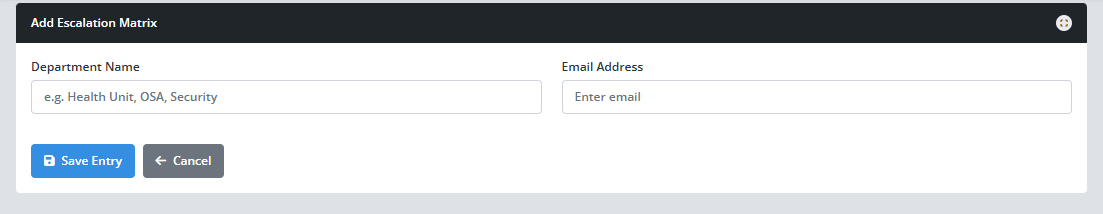
\includegraphics[width=\textwidth]{screenshots/add_escalation_matrix.png}
		\caption{Add Escalation Matrix Form}
	\end{figure}
	
	\section*{View Escalation Matrix Entries}
	After adding entries, they will appear in a tabular format showing:
	\begin{itemize}
		\item Serial number
		\item Department
		\item Email address
		\item Date of creation
	\end{itemize}
	
	\begin{figure}[H]
		\centering
		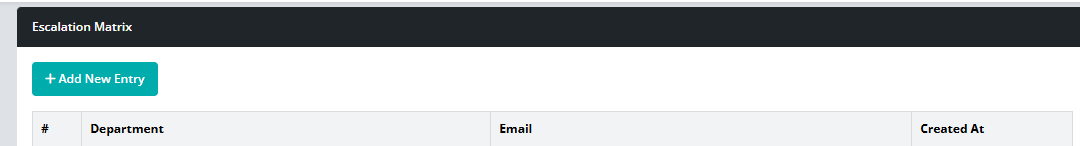
\includegraphics[width=\textwidth]{screenshots/view_escalation_matrix.png}
		\caption{Escalation Matrix List}
	\end{figure}
	
	
	\chapter{Escalations}
	
	\section*{Overview}
	The Escalation module enables users to report and forward critical issues to higher authorities or designated departments.  
	Administrators and authorized users can both \textbf{view escalated issues} and \textbf{send new escalations}.
	
	\section*{Viewing Escalated Issues}
	The \textbf{Escalated Issues} page displays a table of all previously reported escalations.  
	Each entry includes:
	\begin{itemize}
		\item \textbf{\#}: Serial number
		\item \textbf{Date}: Date and time the escalation was created
		\item \textbf{Occurrence ID}: Reference to the related occurrence
		\item \textbf{Recipient}: Email of the escalation recipient
		\item \textbf{Subject}: Subject line of the escalation
		\item \textbf{Message}: The body of the escalation (truncated in the list)
		\item \textbf{Sent By}: The user who created the escalation (or \emph{System})
	\end{itemize}
	
	\begin{figure}[H]
		\centering
		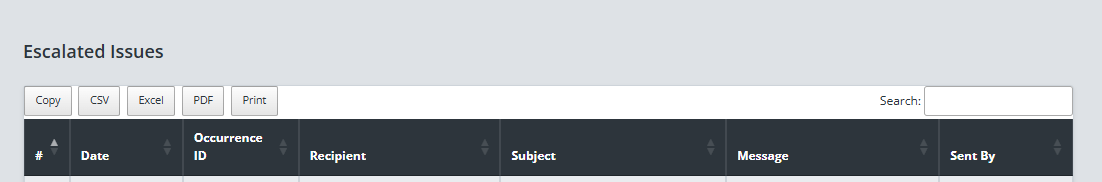
\includegraphics[width=\textwidth]{screenshots/escalated_issues.png}
		\caption{Escalated Issues List}
	\end{figure}
	
	\section*{Sending a New Escalation}
	To create a new escalation:
	\begin{enumerate}
		\item Click the \textbf{Escalate an Issue} button from the relevant page.
		\item Select a \textbf{Recipient} from the dropdown (department or individual email).
		\item Enter the \textbf{Subject}.
		\item Write the \textbf{Message} describing the issue in detail.
		\item Click \textbf{Send Escalation}.
	\end{enumerate}
	
	\begin{figure}[H]
		\centering
		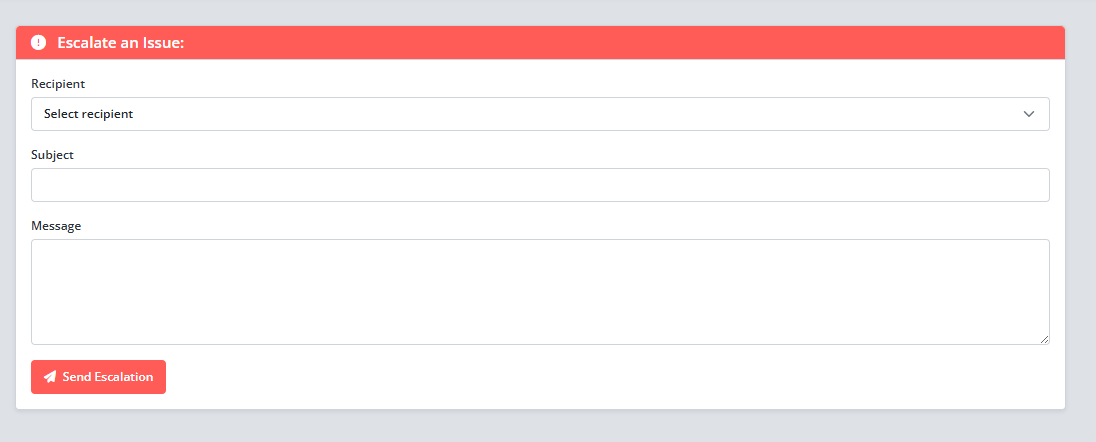
\includegraphics[width=\textwidth]{screenshots/escalate_issue.png}
		\caption{Escalation Form}
	\end{figure}
	
	\chapter{Dashboard}
	
	\section*{Overview}
	The Dashboard provides a quick summary of all important system data in a visual format. 
	It consists of \textbf{widgets} (summary cards with counts) and \textbf{weekly reports} (detailed hostel and zonal statistics). 
	Each widget is clickable, leading to the respective detailed page.
	
	\section*{Dashboard Widgets}
	The top section of the dashboard contains several widgets, including:
	
	\begin{itemize}
		\item \textbf{Total Occurrences}: Displays the total number of all occurrences logged across hostels.
		\item \textbf{Unresolved Issues}: Shows the number of issues pending resolution.
		\item \textbf{Today's Reports}: Indicates how many daily reports were logged today.
		\item \textbf{Hostel Attendants/House Keepers}: Displays the total number of active attendants and keepers.
		\item \textbf{Hostels Covered}: Shows the number of hostels registered in the system. Clicking this expands a breakdown table of students present per hostel.
		\item \textbf{Daily Stats Submitted}: The number of student statistics submitted today.
		\item \textbf{Administrator Reports}: Total reports submitted by administrators today.
		\item \textbf{Zonal Officer Reports}: Total number of zonal reports submitted today. Clicking this expands a detailed breakdown per zone.
	\end{itemize}
	
	\begin{figure}[H]
		\centering
		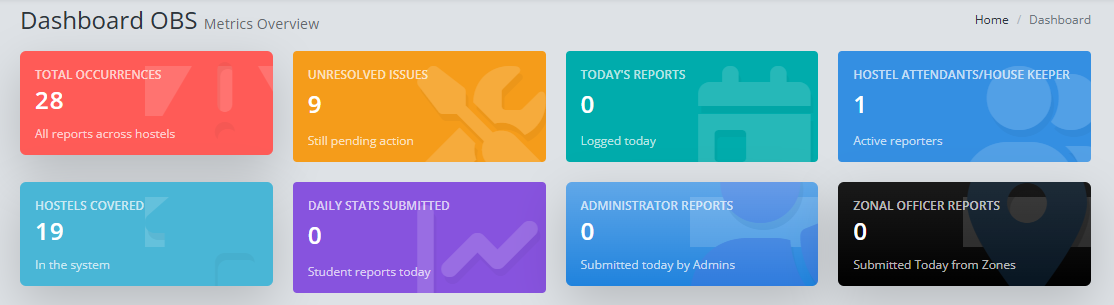
\includegraphics[width=\textwidth]{screenshots/dashboard_widgets.png}
		\caption{Dashboard Widgets Overview}
	\end{figure}
	
	\section*{Weekly Hostel Occupancy Report}
	Below the widgets, the system displays the \textbf{Weekly Hostel Occupancy Report}. 
	This table summarizes hostel capacity, daily occupancy (both \textbf{N}ight and \textbf{D}ay counts), and availability. 
	Navigation buttons allow moving to the previous or next week.
	
	\begin{figure}[H]
		\centering
		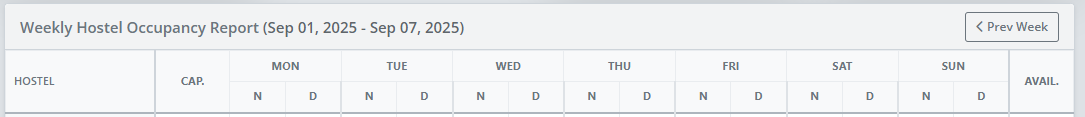
\includegraphics[width=\textwidth]{screenshots/weekly_hostel_report.png}
		\caption{Weekly Hostel Occupancy Report}
	\end{figure}
	
	\section*{Weekly Zonal Occupancy Report}
	The \textbf{Weekly Zonal Occupancy Report} presents similar data, but grouped by zones instead of hostels. 
	It shows total zone capacity, daily occupancy, and available space. 
	Totals across all zones are displayed at the bottom of the table.
	
	\begin{figure}[H]
		\centering
		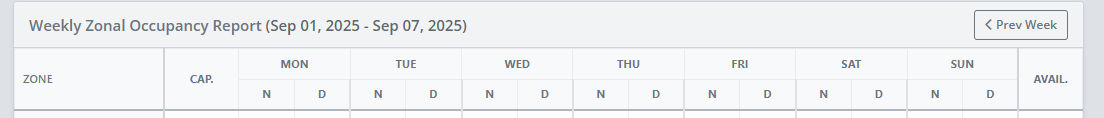
\includegraphics[width=\textwidth]{screenshots/weekly_zonal_report.png}
		\caption{Weekly Zonal Occupancy Report}
	\end{figure}
	
	
	
\end{document}
